\chapter{Análise de tecnologias e ferramentas}
No desenvolvimento deste trabalho foram usados as seguintes ferramentas e tecnologias.

\section{RaspberryPI}
O RaspberryPI é um computador com dimensões reduzidas, do tamanho de um cartão de crédito, que disponibiliza diversos IO para integração. Escolhido por oferecer um bom poder de processamento (que impacta no tempo de resposta dos acionamentos), apresentar um baixo custo e de fácil aquisição no mercado local. É a central de controle do projeto, onde ficam hospedados os serviços e os aplicativos deste projeto, a figura \ref{raspberryPI} mostra uma placa de forma esquemática. \cite{RaspberryPI2017}

\begin{figure}[H]
\caption{\label{raspberryPI}Diagrama esquemático de uma RaspberryPI}
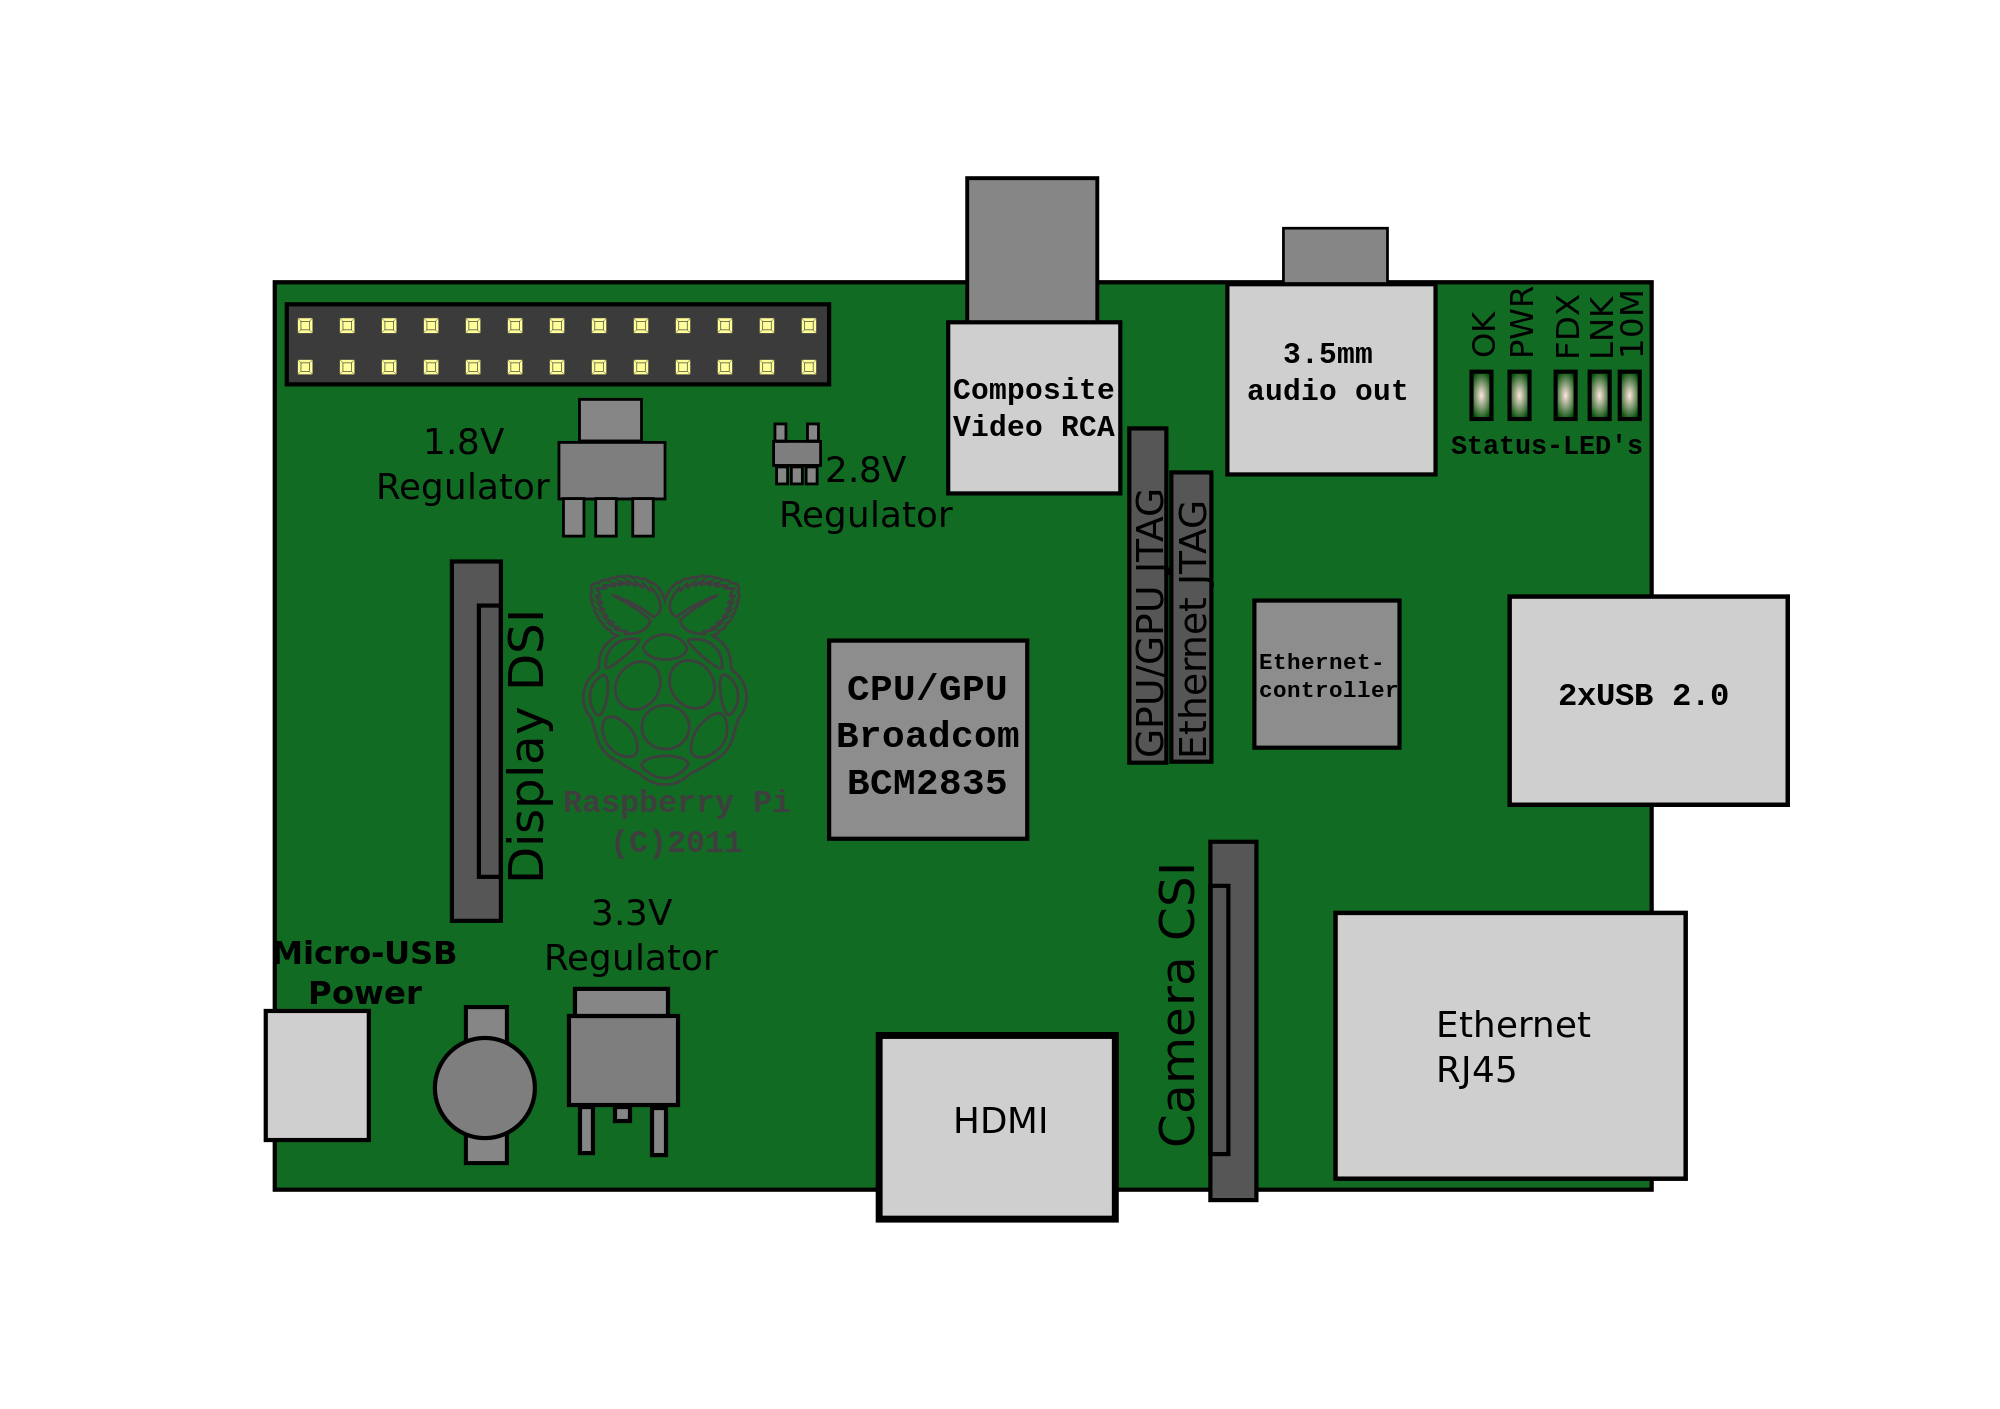
\includegraphics[scale=0.15]{img/raspberrypi.png}
\legend{Fonte: Wikipedia}
\end{figure}

\section{ESP8266}
O ESP8266 é um System-On-Chip (SOC) com WIFI embutido, é produzido pela empresa Espressif, disponibiliza diversos IO e é compatível com o \textit{framework} do Arduíno. (Epressif, 2017). Neste projeto, funciona como um acoplamento a eletrodomésticos existentes, trazendo um interface de comunicação WIFI para dispositivos que não a possuem, é o chamado Módulo Auxiliar (MA), a figura \ref{esp8266} mostra o modelo 01 desta placa e sua pinagem. \cite{Esp82662017}

\begin{figure}[H]
\caption{\label{esp8266}Diagrama esquemático de uma ESP8266-01}
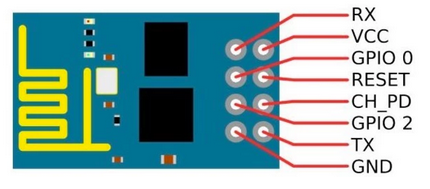
\includegraphics[scale=0.5]{img/esp8266-01f.png}
\legend{Fonte: Autor do projeto}
\end{figure}

\section{Arduíno}
Segundo definição do site Embarcados:

\begin{citacao}
Arduíno é uma plataforma de código aberto (hardware e software) criada em 2005 pelo italiano Massimo Banzi (e outros colaboradores) para auxiliar no ensino de eletrônica para estudantes de design e artistas. O objetivo principal foi o de criar uma plataforma de baixo custo, para que os estudantes pudessem desenvolver seus protótipos com o menor custo possível. Outro ponto interessante do projeto, foi a proposta de criar uma plataforma de código aberto, disponível para a comunidade o que ajudou em muito no seu desenvolvimento. \cite{OQUEARDUINO}
\end{citacao}

Foi a ferramenta escolhida para o desenvolvimento do \textit{firmware} do Módulo Auxiliar (MA) em função da facilidade de uso e por oferecer um grande número de bibliotecas para os mais diversos hardwares de mercado. \cite{Arduino2017}

\section{Javascript}
Javascript é a principal linguagem de programação para desenvolvimento de aplicativos para browsers de internet. É utilizada para o desenvolvimento da interface com usuário final. 

\section{Python}
Segundo o site do projeto:

\begin{citacao}
Python é uma linguagem de programação de alto nível, interpretada, de script, imperativa, orientada a objetos, funcional, de tipagem dinâmica e forte.  \cite{PYTHON}
\end{citacao}

Foi a alternativa encontrada, quando dos problemas de performance na utilização de NodeJS \cite{NodeJS2017}. Em um período curto de tempo, quatro dias, toda API para controlar os módulos auxiliares foi reescrita.

\section{SQLite}
A wikipedia faz uma tradução do site do projeto, segundo eles:

\begin{citacao}
SQLite é uma biblioteca em linguagem C que implementa um banco de dados SQL embutido. Programas que usam a biblioteca SQLite podem ter acesso a banco de dados SQL sem executar um processo Sistema de Gerenciamento de Banco Dados (SGBD) separado. \cite{SQLITE}
\end{citacao}
Foi a opção escolhida devido a performace e falicidade de implementação para ambientes com Linux embarcado.

\section{MQTT}
MQTT é um protocolo de comunicação do tipo Machine to Machine (M2M) desenvolvido pela IBM no inicio dos anos 2000 como solução de comunicação entre hardwares de baixa capacidade de computação de dados com equipamentos mais robustos. Este protocolo serve de "cola" entre todos os entes de um sistema heterogêneo, onde servidores, computadores pessoais, smartfones e microcontroladores precisam conversar. Neste projeto é utilizado como o meio de comunicação entre todos os MAs e a central de controle. \cite{Mqtt2017}

\section{Mosquitto}
Mosquitto é um Broker, ou central de controle de mensagens, que utiliza o protocolo MQTT para troca de mensagens em dispositivos diversos sobre o protoclo TCP. Está instalado e configurado como serviço na RaspberryPI portanto, fazendo parte da central de controle.\cite{MOSQUITTO}

\section{Debian Linux}
Debian Linux é uma das primeiras distribuições Linux 1993, conhecido por seu rigoroso critério na aprovação de pacotes e na consequente robustez do sistema. Oferece uma licença para uso pessoal ou comercial que não onera o projeto. É o sistema operacional da central de controle. \cite{Debian2017}

\section{Geany IDE}
Segundo o site do projeto, Geany é um editor de textos que usa o kit gráfico GTK+ com características básicas de uma \textit{Integrated Development Environment} (IDE), tradução do autor. Todo o código escrito neste projeto usou esta IDE. \cite{GEANY2017}

\section{Schemacrawler}
Segundo o site do projeto, Schemacrawler é uma ferramenta de descoberta e compreensão de esquemas de banco de dados, tradução do autor. Esta ferramenta foi utilizada para a partir do banco de dados gerado pelo módulo de \textit{Object-relational mapping} (ORM), mapear as tabelas e relacionamentos, traduzindo para um diagrama Entidade Relacionamento. \cite{CRAWLER}

\section{Git SCM}
Segundo o site do projeto, Git é um sistema de controle distribuído de código fonte aberto, projetado para lidar com tudo, de pequenos a grandes projetos com velocidade e eficiência, tradução do autor. Todo material deste projeto incluindo este relatório estão versionados e controlados com o Git. \cite{GIT2017}

\section{Gliffy}
Gliffy é uma extensão do google chrome para criação e edição de diagramas, usada neste projeto para elaboração dos diagramas de BPM e fluxo de dados. \cite{GLIFFY}

\section{VueJS}
Vuejs é um framework \textit{open-source} utilizado para desenvolvimento de interfaces gráficas para ambientes web. Foi escolhido para este projeto devido a simplicidade e facilidade de uso, envolve um \textit{setup} de ambiente de desenvolvimento que requer poucos recursos(é possível iniciar o desenvolvimento sem o uso de NodeJS e sua coleção de ferramentas). Separa o tratamento de dados da visualização destes o que facilita a modularização do projeto. \cite{VUEJS}

\section{Skeleton}
Skeleton é um \textit{template} para desenvolvimento de interfaces web, oferece uma estrutura miníma de html e css. Foi a opções escolhida em função do tamanho reduzido, da simplicidade para iniciar o desenvolvimento e rapidez em obter resultados. \cite{SKELETON}
